\documentclass{article}

\usepackage[utf8x]{inputenc}
\usepackage[portuguese]{babel}
\usepackage[linesnumbered,ruled,vlined]{algorithm2e}
\usepackage{algpseudocode}
\usepackage{xcolor}
\usepackage{graphicx}
\usepackage{cite}
\usepackage{listings}
\newcommand\bruno[1]{({\color{red}#1})}
\newcommand\philippe[1]{({\color{blue}#1})}

\title{Compiler C to PDL}
\date{09-08-2018}
\author{Philippe Geraldeli Araujo e Allan Patrick}
\newtheorem{definicao}{Definição}

\begin{document}
	
	\maketitle
	\pagenumbering{gobble}
	\newpage
	\pagenumbering{arabic}
	
	\section{C to PDL}
	
	\paragraph{Fork do miniC feito por eubnara\\}
	Este compilador tem o objetivo de converter C para PDL(Propositional Dynamic Logic). \vspace{10mm}
	
	\small \bruno{Verifiquem o que os caracteres especiais dessa gramática significa.	\philippe{Não achei nada referente a essa extensão do BNF, estou entrando em contato com o eubnara para saber mais sobre isso, se for o caso refatoro}} 
	\noindent
	Program := (DeclList)? (FuncList)?   \\
	DeclList := (Declaration)+          \\
	FuncList := (Function)+ \\ 
	Declaration := Type IdentList \\
	IdentList := identifier (, identifier)* \\
	Identifier := id ou id [ intnum ]       \\
	Function := Type id ( (ParamList)? ) CompoundStmt \\
	ParamList := Type identifier (, Type identifier)* \\
	Type := int ou float \\
	CompoundStmt := { (DeclList)? StmtList } \\
	StmtList := (Stmt)* \\
	Stmt := AssignStmt ou CallStmt ou RetStmt ou WhileStmt ou ForStmt ou IfStmt ou CompoundStmt ou ; \\
	AssignStmt :=Assign  \\
	Assign := id = Expr ou id [ Expr ] = Expr \\
	CallStmt := Call ; \\
	Call := id ( (ArgList)? ) \\
	RetStmt := return (Expr)? ;  \\
	Expr := MINUS Expr $|$ MathRel Eqltop Expr $|$ MathRel $|$ Call $|$ Ids \\
	MathRel := MathEql Relaop MathRel $|$ MathEql \\
	MathEql := TERM Addiop MathEql $|$ TERM \\
	TERM := FACTOR Multop TERM $|$ FACTOR \\
	FACTOR := '(' Expr ')' $|$ FLOATNUM $|$ INTNUM \\
	Id := ID $|$ ID [ Expr ] \\
	
	
	O nosso programa não segue a regra abaixo:  \\
	1. ++, --  \\
	2. De acordo com essa regra  :=  CompoundStmt := { (DeclList)? StmtList }  \\
	
	\section{Algorithm Converter} \bruno{Tá uma mistureba de inglês e português. Definam um único idioma. 	\philippe{o codigo tá em ingles, o algoritmo em portugues, se quiser refatoro pra tudo em ingles}} \\
	Entrada = Arquivo em C \\
	Saída = Arvore/Arquivo
	\vspace{10mm}
	
	\begin{algorithm}
		
		\caption{BuildTree(Program* head)}
		
		\If{headDeclaration != NULL}{
			visitDeclaration(headDeclaration)\;
		}
		\If{headFunction != NULL}{
			visitFunction(headFunction)\;
		}
		
	\end{algorithm}
	
	\BlankLine
	
	\begin{algorithm}
		\caption{visitDeclaration(DECLARATION* decl)}
		
		\If{DeclList}{
			\If{Declaration}{
				insert(declarationType)\;
				insert(declarationId)\;
				
			}
			\If{DeclList}{
				visitDeclaration(previousDeclaration)\;
			}
		}
		
		
		
		
	\end{algorithm}
	\begin{algorithm}
		
		\caption{visitFunction(FUNCTION* func)}
		
		\If{FunctionList}{
			\If{FunctionList}{
				visitFunction(previousFunction)\;
			}
			\If{Function}{
				insert('(')\;
				\If{funcParameter != NULL}{
					insert(funcParameter)\;
				}
				visitCompoundStmt(FunctionCstmt)\;
			}
		}
		
		
		
		
	\end{algorithm}
	
	\begin{algorithm}
		
		\caption{visitCompoundStmt(COMPOUNDSTMT* cstmt)}
		
		\If{cstmtDeclaration != NULL}{
			visitDeclaration{cstmtDeclaration}\;
		}
		\If{cstmtStatement != NULL}{
			visitStmt(cstmtStatement)\;
		}
		
	\end{algorithm}
	
	\begin{algorithm}[H]
		
		\caption{visitStmt(Stmt* stmt)}
		
		\Switch{stmtS}{
			\Case{Assign}{
				InsertSemicolon()\;
				insert(stmtS\_AssignID)\;
				insert("=")\;
				insert(stmtS\_AssignExpression)\;
			}
			\Case{Call}{
				insertSemicolon()\;
				insert(stmtSCallIdentifier)\;
				insert(CallArg)\;
			}
			\Case{Return}{
				\eIf{Stmt\_Return == NULL}{
					insert("return")\;
				}{
					insert("return")\;
					visitStmt(stmtS\_Return)\;
				}
			}
			\Case{While}{
				\eIf{StmtSdo\_while == true}{
					visitStmt(stmtS\_while)\;
					insert(WhileCondition)\;
					visitStmt(stmtS\_while)\;
					insert(")*;$\neg$(")\;
				}{
					insert(WhileCondition)\;
					visitStmt(stmtS\_while)\;
					insert(")*$\neg$")\;
					insert(WhileCondition)\;
				}
			}
			\Case{For}{
				visitStmtS(StmtSAssign)\;
				insert(ForCondition)\;
				visitStmt(stmtS\_For)\;
				visitStmt(stmtS\_ForInc)\;
				insert(ForCondition)\;
				
			}
			\Case{If}{
				insert(If\_condition)\;
				VisitStmt(stmtS\_if)\;
				\If{stmtSelse != NULL}{
					insert(IfCondition)\;
					%visitExpr(stmtScondition)\;
					visitStmt(stmtSelse)\;
				}
			}
			\Case{CompoundStmt}{
				visitCompoundStmt{stmtS}\;
			}
			\Case{Semicolon}{
				insert("$;$")\;
			}
		}
	\end{algorithm}
	
	
	\section{Prova de corretude do algoritmo:}
	\BlankLine
	O Propositional Dynamic Logic(PDL) é uma lógica completa, isto é, se existir um caminho correto, iremos chegar até ele. Porém, precisamos partir da hipótese que o programa sempre vai parar. Nesse algoritmo foi utilizado o Flex e o Bison como ferramentas, nele é gerado uma árvore de execução que segue o Formalismo de Backus-Naur(BNF) apresentado no capitulo 1. O algoritmo então opera nessa árvore, que por sua vez é construída com a estratégia ``bottom-top". Sendo assim, todo caso é tratado isoladamente, isto é, se todo caso base é comprovadamente correto, a composição deles também é. Temos então os casos das estruturas de repetição, condição e escopo. A condição de escopo é a mais simples, pois como em PDL é ignorada, um escopo é estruturado toda vez que a recursão entra em uma função, logo esse caso é ignorado pela conversão. Assim mostraremos que para um caso genérico Sigma de um subconjunto da linguagem C todas as transformações feitas são válidas, já que é comprovado que todas as conversões de uma linguagem de programação para PDL estão corretas. Agora iremos mostrar que o algoritmo de conversão gera um resultado equivalente a conversão que já está comprovada.
	\BlankLine
	
	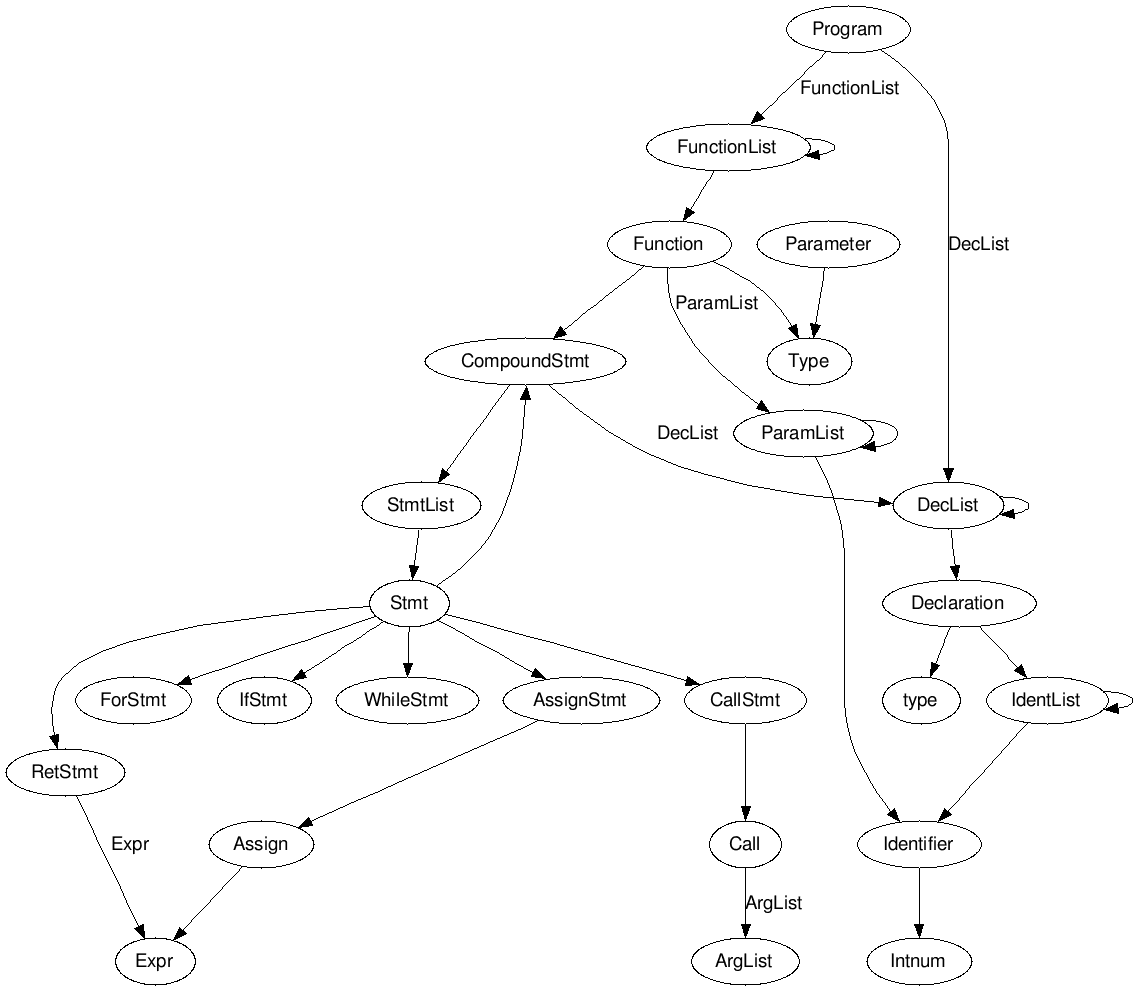
\includegraphics[width=\textwidth]{Arvore}
	\\
%	\bruno{Explicar inicialmente o algoritmo. Quais as hipóteses e definições utilizadas? Explicitem que o parser foi construído com Flex + Bison que geraram uma árvore e é sobre ela que vocês operam. Apresentem a forma dessa árvore. Exemplos de entrada não devem ser apresentados como algoritmos, usem outro ambiente como listings.}
	
	\BlankLine
	Uma estrutura de Assign por exemplo se comporta do seguinte modo:\\
	
	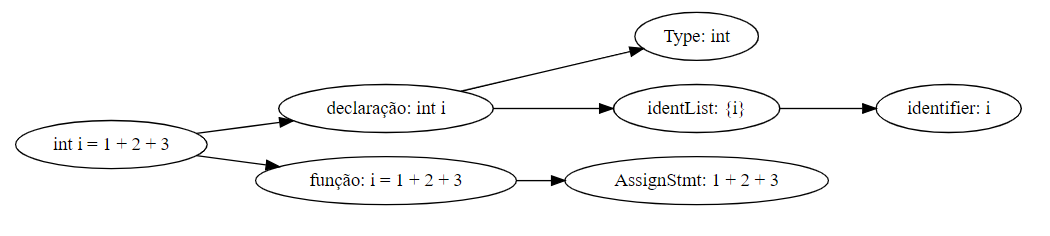
\includegraphics[width=\textwidth]{assignStmt}
	\BlankLine
	
	\subsection{Estruturas de condição} 
	Todas as definições a seguir são explicitadas em\cite{PDL}. 
	\BlankLine 
	\flushleft
	A conversão para PDL de um \texttt{if} simples ocorre assim: 
	%\bruno{Não forcem quebra de linha sem necessidade. Deixem o \LaTeX\ cuidar da formatação. Observem que alterei a tipografia do ``if'' para ficar mais fácil de ler. Adotem uma tipografia específica e apliquem no documento.}
	\begin{definicao}%\bruno{De onde vem essa definição? Criem uma única definição com todas as formas utilizadas.}
		If $\varphi$ then $\alpha$ else $\beta$ $\rightarrow$ $\varphi$? ; $\alpha$ $\cup \neg\alpha$? ; $\beta$
	\end{definicao}
	
	 O compilador faz essa conversão da seguinte forma:\\
	
	\BlankLine
	\begin{algorithm}[H]
		\KwData{Codigo em c}
		\KwResult{Programa em PDL correspondente ao if}
		\caption{(void visitIf\_s2(struct IF\_S* if\_s))}
		scopeTail = newScope(sIF, scopeTail)\;
		\_isTitlePrinted2 = false\;
		scopeTail$\rightarrow$parent$\rightarrow$if\_n++\;
		
		insert(aux, "child", "( (")\;
		aux2 = aux\;
		visitExpr2(if\_s$\rightarrow$cond)\;
		insert(aux,"child",")? ")\;
		\If{if\_s$\rightarrow$if\_$\rightarrow$s}{
			insert(aux,"child",";")\;
		}
		visitStmt2(if\_s$\rightarrow$if\_)\;
		insert(aux,"child"," )")\;
		\If{if\_s$\rightarrow$else\_ != NULL}{
			insert(aux, "child", "$\cup$($\neg$(")\;
			aux2 = aux\;
			visitExpr2(if\_s$\rightarrow$cond)\;
			insert(aux,"child",")? ")\;
			\If{if\_s$\rightarrow$else\_$\rightarrow$s}{
				insert(aux,"child",";")\;
			}
			visitStmt2(if\_s$\rightarrow$else\_)\;
			insert(aux, "child", ")")\;
		}
	\end{algorithm}
	\begin{flushleft}
	Na linha 4 adiciona dois escopos de parêntese na árvore. \\
	Na linha 6 procura a condição do if para adicionar em seguida no visitExpr2. \\
	Na linha 7 fecha o parêntese e adiciona o “?”.\\
	Na linha 10 vai para o Stmt do if\\
	Nessa etapa do programa temos um \texttt{If} simples, sendo $\varphi$ = cond e $\alpha$ = Stmt temos então: ($\varphi$? ; $\alpha$) \\
	Na linha 13 é checado se existe um else, caso exista é adicionado o “$\cup$\label{key}($\neg$(“ na  linha 12. \\
	Na linha 17 é adicionado a condição novamente.\\
	Na linha 18 termina o escopo do if.\\	
	Percebe-se que da mesma forma que a etapa anterior, o else possui o mesmo comportamento, porém com uma negação, sendo o stmt do else igual a $\beta$, temos:\\ (($\varphi$? ; $\alpha$) $\cup   (\neg\alpha$? ; $\beta$)) \\ 
	
	\end{flushleft}%\bruno{Aqui vocês explicam como a construção é feita, mas falta deixar claro que isso corresponde a definição do programa PDL adotada.}
	Logo, podemos perceber que os dois casos de \texttt{If} são equivalentes %\bruno{O que significa ser trivialmente equivalente? Entendo que aqui vocês tentaram fazer o que pedi acima, mas não está claro.} 
	aos casos que ocorrem na definição de PDL. O algoritmo faz essa conversão e insere na árvore os possíveis casos gerando ramificações. Assim levando ao caso base de cada ramificação e sendo tratada pela recursão.

	\subsection{Caso Call}
	\BlankLine
	Ao passar pela função o compilador cria diferentes árvores. Cada árvore tem seu nome armazenado como uma tag, sendo assim, quando uma função é chamada é adicionada essa tag na conversão referenciando a árvore em questão.	 
	
	%Nesse caso o que estamos fazendo na prática é nada mais nada menos \bruno{Isso é um documento, não uma conversa. Evitem esse tipo de colocação em textos formais.} que entrando em uma função normalmente, logo quando temos a chamada de uma função externa é fácil ver que é apenas uma função que será inserida na árvore normalmente. 
	
	\subsection{Estruturas de repetição} %\bruno{Em vez de ``*'' usem ``$^\star$''.}
	O $^\star$ no PDL significa que o escopo é repetido zero ou mais vezes, logo não temos controle de quantas iterações serão executadas no programa, mas sabemos que é um numero finito de vezes. Assim, essa abstração as vezes pode significar uma perda parcial de expressividade.\\
	\subsubsection{Caso While e doWhile}
	Temos que a conversão de um while para PDL ocorre da seguinte forma de acordo com a definição:\\
	
	\begin{definicao}
		While $\varphi$ do $\beta$ $\rightarrow$ ($\varphi$? ; $\beta$)$^\star$ ; $\neg$$\varphi$?
	\end{definicao}
	
	\begin{definicao}
		do $\beta$ While $\varphi$ $\rightarrow$  $\beta$ ;(($\varphi$? ; $\beta$)$^\star$ ; $\neg$$\varphi$?)
	\end{definicao}
	Temos então o algoritmo do while:\\
	
	\begin{algorithm}[H]
		
		\KwData{Codigo em c}
		\KwResult{Programa em PDL correspondente ao while ou doWhile}
		\eIf{while\_s$\rightarrow$do\_while == true}{
			insert(aux, "child", "(")\;
			visitStmt2(while\_s$\rightarrow$stmt)\;
			insert(aux, "child", "(")\;
			aux2 = aux\;
			visitExpr2(while\_s$\rightarrow$cond)\;
			insert(aux,"child",")?")\;
			visitStmt2(while\_s$\rightarrow$stmt)\;
			insert(aux, "child", ")*;$\neg$(")\;
			aux2 = aux\;
			visitExpr2(while\_s$\rightarrow$cond)\;
			insert(aux,"child",")? ")\;
		}{
			insert(aux, "child", "( (")\;
			aux2 = aux\;
			visitExpr2(while\_s$\rightarrow$cond)\;
			insert(aux,"child",")?")\;
			visitStmt2(while\_s$\rightarrow$stmt)\;
			insert(aux, "child", ")*;$\neg$(")\;
			aux2 = aux\;
			visitExpr2(while\_s$\rightarrow$cond)\;
			insert(aux,"child",")?")\;
		}
	\end{algorithm}
	\begin{flushleft}
	Nas linhas 1,12 é feito um teste para saber se é um dowhile ou um while, no caso de ser um do while ele irá continuar na linha 2, caso contrário na linha 12.\\
	Na linha 2 é inserido um parêntese.\\
	Na linha 3 é adicionado tudo que possui dentro do while.\\
	Nessa etapa como é adicionado a execução do programa temos: $\beta$
	
	Na linha 4 é feita mais uma adição de parêntese.\\
	Na linha 6 é adicionada a condição do dowhile.\\
	Na linha 8 é tratada da forma de um while normal.\\
	\BlankLine
	A partir desse processo temos que o programa PDL formado sendo $\varphi$ a condição e $\beta$ o stmt equivale a: ($\beta$ ;(($\varphi$? ; $\beta$)$^\star$ ; $\neg$$\varphi$?)) \\
	\BlankLine
	Na linha 14 é adicionado 2 parênteses.\\
	Na linha 15 é adicionada a condição do while.\\
	Na linha 17 se fecha o parênteses e adiciona o “?”. \\
	Na linha 18 é adicionado tudo que o while possui internamente.\\
	Na linha 19,21,22 é adicionado a negação da condição e adicionado um ponto de interrogação.\\
	Tendo como condição e stmt o mesmos simbolos temos:  ($\varphi$? ; $\beta$)$^\star$ ; $\neg$$\varphi$?)\\
	
	\end{flushleft} %\bruno{Vide comentários anteriores e apliquem no que segue, também.}
	
	Logo, podemos afirmar que a partir da execução desse algoritmo temos a conversão em PDL do While/doWhile, pois há equivalência no programa gerado pelo algoritmo e a definição citada.
	\subsubsection{Caso For}
	
	O for também pode ser tratado da mesma forma que o while, mas com algumas ressalvas. Logo a conversão de for para PDL ocorre da seguinte forma: no ``for" temos 3 campos, o de declaração, condição e incremento. Sendo ``decl" a declaração, ``cond" a condição e ``inc" o incremento, temos como exemplo:\\
	
\begin{lstlisting}[frame=single]  % Start your code-block

for (decl ; cond ; inc){
	stmt
}

\end{lstlisting}

	
	Assim, a conversão é equivalente a um while e é feita da seguinte forma:\\
	\BlankLine	
	decl ; ((cond? ; stmt ; inc)* ; $\neg$cond?)\\
	\BlankLine
	

	
	\begin{algorithm}
		
		\KwData{Codigo em c}
		\KwResult{Programa em PDL correspondente ao for}
		\caption{visitFor\_s2 (struct FOR\_S* for\_s)}
		insert(aux, "child","(")\;
		visitAssignStmt2(for\_s$\rightarrow$init)\;
		insert(aux,"child",";(")\;
		aux2 = aux\;
		visitExpr2(for\_s$\rightarrow$cond)\;
		insert(aux,"child",")?")\;
		insert(aux, "child", "; ")\;
		visitStmt2(for\_s$\rightarrow$stmt)\;
		insert(aux,"child", "; ")\;
		visitAssignStmt2(for\_s$\rightarrow$inc)\;
		insert(aux,"child",")*;$\neg$(")\;
		aux2 = aux\;
		visitExpr2(for\_s$\rightarrow$cond)\;
		insert(aux,"child",")?$\neg$for\_s$\rightarrow$cond")\;
	\end{algorithm}
	\begin{flushleft}
	Na linha 1 é adicionado um parêntese.\\
	Na linha 2 é adicionado a declaração dentro do for, dado como “for\_s$\rightarrow$init”\\
	Na linha 3 é adicionado mais um parêntese.\\
	Na linha 5 é adicionada toda a condição do for.\\
	Na linha 6 se fecha o parêntese da condição do for.\\
	Na linha 8 é adicionado tudo que estava dentro do for.\\
	Na linha 10 é adicionado o campo de incremento.\\
	
	Seja a declaração um programa $\pi$, a condição $\varphi$, o incremento $\varpi$, e o stmt $\vartheta$, temos:
	
	($\pi$ ; ($\varphi$? ; $\varpi$ ; $\vartheta$)$^\star$)
		\end{flushleft}
	\vspace{25mm}
	Logo, podemos verificar trivialmente que a equivalência a um while com uma declaração e um incremento e a conversão do compilador são equivalentes. Portanto, pode-se concluir que a corretude do for do compilador está correta visto que a corretude de conversão para o pdl também está correta.Por fim como estes elementos englobam todo o escopo do subconjunto de c utilizado pelo algoritmo temos que a corretude do mesmo está correta visto que a corretude de cada elemento está correta.\\
	

	\begin{thebibliography}{00}

		\bibitem{PDL}
		M.J. Fischer, R.E. Ladner, Propositional dynamic logic of regular programs, J. Comput. System Sci.18 (2):194-211, 1979
		
	\end{thebibliography}
\end{document}

